%%%% Thanks to A. Gupta and R. Ravi for providing this template file.



\documentclass[11pt]{article}
\usepackage{amsfonts}
\usepackage{amssymb}
\usepackage{amstext}
\usepackage{amsmath}
\usepackage{xspace}
\usepackage{theorem}
\usepackage{color}
\usepackage[pdftex]{graphicx}
\usepackage{epsfig}
\usepackage[ruled,algosection,vlined,linesnumbered]{algorithm2e}
\usepackage{tikz}
%\usepackage{layout}% if you want to see the layout parameters
                     % and now use \layout command in the body

% This is the stuff for normal spacing
\makeatletter
 \setlength{\textwidth}{6.5in}
 \setlength{\oddsidemargin}{0in}
 \setlength{\evensidemargin}{0in}
 \setlength{\topmargin}{0.25in}
 \setlength{\textheight}{8.25in}
 \setlength{\headheight}{0pt}
 \setlength{\headsep}{0pt}
 \setlength{\marginparwidth}{59pt}

 \setlength{\parindent}{0pt}
 \setlength{\parskip}{5pt plus 1pt}
 \setlength{\theorempreskipamount}{5pt plus 1pt}
 \setlength{\theorempostskipamount}{0pt}
 \setlength{\abovedisplayskip}{8pt plus 3pt minus 6pt}

 \renewcommand{\section}{\@startsection{section}{1}{0mm}%
                                   {2ex plus -1ex minus -.2ex}%
                                   {1.3ex plus .2ex}%
                                   {\normalfont\Large\bfseries}}%
 \renewcommand{\subsection}{\@startsection{subsection}{2}{0mm}%
                                     {1ex plus -1ex minus -.2ex}%
                                     {1ex plus .2ex}%
                                     {\normalfont\large\bfseries}}%
 \renewcommand{\subsubsection}{\@startsection{subsubsection}{3}{0mm}%
                                     {1ex plus -1ex minus -.2ex}%
                                     {1ex plus .2ex}%
                                     {\normalfont\normalsize\bfseries}}
 \renewcommand\paragraph{\@startsection{paragraph}{4}{0mm}%
                                    {1ex \@plus1ex \@minus.2ex}%
                                    {-1em}%
                                    {\normalfont\normalsize\bfseries}}
 \renewcommand\subparagraph{\@startsection{subparagraph}{5}{\parindent}%
                                       {2.0ex \@plus1ex \@minus .2ex}%
                                       {-1em}%
                                      {\normalfont\normalsize\bfseries}}
\makeatother

\newenvironment{proof}{{\bf Proof:  }}{\hfill\rule{2mm}{2mm}}
\newenvironment{proofof}[1]{{\bf Proof of #1:  }}{\hfill\rule{2mm}{2mm}}
\newenvironment{proofofnobox}[1]{{\bf#1:  }}{}\newenvironment{example}{{\bf Example:  }}{\hfill\rule{2mm}{2mm}}
\renewcommand{\thesection}{\lecnum.\arabic{section}}

\renewcommand{\theequation}{\thesection.\arabic{equation}}
\renewcommand{\thefigure}{\thesection.\arabic{figure}}

\newtheorem{fact}{Fact}[section]
\newtheorem{lemma}[fact]{Lemma}
\newtheorem{theorem}[fact]{Theorem}
\newtheorem{definition}[fact]{Definition}
\newtheorem{corollary}[fact]{Corollary}
\newtheorem{proposition}[fact]{Proposition}
\newtheorem{claim}[fact]{Claim}
\newtheorem{exercise}[fact]{Exercise}
\newtheorem{note}[fact]{Note}

% math notation
\newcommand{\R}{\ensuremath{\mathbb R}}
\newcommand{\Z}{\ensuremath{\mathbb Z}}
\newcommand{\N}{\ensuremath{\mathbb N}}
\newcommand{\F}{\ensuremath{\mathcal F}}

\newcommand{\size}[1]{\ensuremath{\left|#1\right|}}
\newcommand{\ceil}[1]{\ensuremath{\left\lceil#1\right\rceil}}
\newcommand{\floor}[1]{\ensuremath{\left\lfloor#1\right\rfloor}}

\DeclareMathOperator{\conv}{conv}
\DeclareMathOperator{\cone}{cone}
\DeclareMathOperator{\aff}{aff}
\DeclareMathOperator{\rec}{rec}
\DeclareMathOperator{\lin}{lin}
\DeclareMathOperator{\rank}{rank}



%%%%%%%%%%%%%%%%%%%%%%%%%%%%%%%%%%%%%%%%%%%%%%%%%%%%%%%%%%%%%%%%%%%%%%%%%%%
% Document begins here %%%%%%%%%%%%%%%%%%%%%%%%%%%%%%%%%%%%%%%%%%%%%%%%%%%%
%%%%%%%%%%%%%%%%%%%%%%%%%%%%%%%%%%%%%%%%%%%%%%%%%%%%%%%%%%%%%%%%%%%%%%%%%%%

\newcommand{\headings}[4]{
{\bf CO 759: Topics in Integer Programming} \hfill {{\bf Lecturer:} #1}\\
{{\bf Topic:} #2} \hfill {{\bf Date:} #3} \\
{{\bf Scribe:} #4}\\
\rule[0.1in]{\textwidth}{0.025in}
%\thispagestyle{empty}
}

\begin{document}
\headings{Ricardo Fukasawa}{Decomposition Theorem and Orthogonal Projections}{Jan/12/2016}{William Justin Toth}
\newcommand{\lecnum}{3}

\section{Decomposition}
\subsection{Extreme Points, Vertices, Basic Feasible Solutions}
\paragraph{Extreme Point} Let $P = \{ x : Ax \leq b \} \subseteq \R^n$, and let $\bar{x} \in P$. We say $\bar{x}$ is an $\textit{extreme point}$ of $P$ provided $$\not\exists\ x^1, x^2 \in P \backslash \{\bar{x}\} \text{ such that }\bar{x} = \frac{1}{2}(x^1 + x^2).$$
\begin{note}
An equivalent condition is to say that 
$$\not\exists\ x^1, x^2 \in P \backslash \{\bar{x}\} \text{ such that }\bar{x} = \lambda x^1 + (1-\lambda)x^2 \text{ for some } \lambda \in (0,1).$$
\end{note}
\begin{proof}
Let $P = \{x \in \R^n : Ax \leq b\}$. Let $\bar{x} \in P$.
\paragraph{}
Suppose that there exists $x^1, x^2 \in P\backslash\{x\}$ such that $\bar{x} = \frac{1}{2}(x^1 + x^2)$. Then taking $\lambda = \frac{1}{2} \in (0,1)$ gives that $\bar{x} = \lambda x^1 + (1-\lambda)x^2$ as desired.
\paragraph{}
Now suppose that there exists $x^1, x^2 \in P\backslash\{x\}$ such that $\bar{x} = \lambda x^1 + (1-\lambda)x^2$ for some $\lambda \in (0,1)$. We may assume that $\lambda \leq \frac{1}{2}$ without loss of generality (as otherwise we switch the labels $x^1$ and $x^2$ and proceed). Consider the vector:
$$ a^1 = \frac{1}{2} \lambda x^1 + \frac{2-\lambda}{2} x^2.$$
Since $\frac{1}{2} \lambda + \frac{2-\lambda}{2} = 1$ and $\frac{1}{2}\lambda, \frac{2-\lambda}{2} \geq 0$ we have that $a^1$ is a convex combination of $x^1$ and $x^2$. Since $P$ is a convex set we thus have that $a^1 \in P$. Additionally consider the vector:
$$ a^2 = \frac{3}{2} \lambda x^1 + \frac{2-3\lambda}{2}x^2.$$
Since $\frac{3}{2} \lambda + \frac{2-3\lambda}{2} = 1$ and $\frac{3}{2}\lambda, \frac{2-3\lambda}{2} \geq 0$ (recall we assume that $\lambda \leq \frac{1}{2}$) we have that $a^2$ is a convex combination of $x^1$ and $x^2$. Since $P$ is a convex set we thus have that $a^2 \in P$. Now we compute:
\begin{align*}
\frac{1}{2}(a^1 + a^2) &= \frac{1}{2}(\frac{1}{2}\lambda x^1 + \frac{2-\lambda}{2}x^2 + \frac{3}{2}\lambda x^1 + \frac{2-3\lambda}{2}x^2) \\
&= \frac{1}{2}(2\lambda x^1 + \frac{4-4\lambda}{2}x^2) \\
&=\lambda x^1 + (1-\lambda)x^2 \\
&=\bar{x}.
\end{align*}
Thus there exists $a^1,a^2 \in P$ such that $\bar{x} = \frac{1}{2}(a^1 + a^2)$.
\end{proof}
\paragraph{Basic Feasible Solution} Let $P = \{ x : Ax \leq b \} \subseteq \R^n$, and let $\bar{x} \in P$. We say $\bar{x}$ is a $\textit{basic feasible solution}$ (BFS) provided $\bar{x}$ satisfies $n$ linearly independent constraints of $P$ at equality.
\paragraph{Vertex} Let $P = \{ x : Ax \leq b \} \subseteq \R^n$, and let $\bar{x} \in P$. We say $\bar{x}$ is a $\textit{vertex}$ of $P$ provided  it is a dimension $0$ face of $P$.
\begin{theorem}
If $P \subseteq \R^n$ is a pointed polyhedron then the following are equivalent:
\begin{enumerate}
\item $\bar{x}$ is an extreme point of $P$,
\item $\bar{x}$ is a vertex of $P$,
\item $\bar{x}$ is a BFS,
\item $\exists\ c:\bar{x}$ is the unique optimal solution to $max\{c^Tx : x \in P\}$.
\end{enumerate}
\end{theorem}
\begin{proof}
Omitted.
\end{proof}
\paragraph{}
In the figure below, $\bar{x}$ is an extreme point/vertex/BFS, and $a^1$ and $a^2$ label the lines corresponding to the $2$ linear inequalities satisfied at equality. The points $x^1, x^2$ demonstrate the geometric interpretation of the extreme point definition.
\begin{figure}[ht]
\centering
\begin{tikzpicture} 
\draw [fill=lightgray] (4,1.5) node[right]{$\bar{x}$} -- node[left]{$a^2$}(3,0) -- (1,0) -- (0,1.5) -- (1,3) -- (3,3) -- node[left]{$a^1$}(4,1.5);
\draw [dashed] (4, 2) node[above]{$x^1$} -- (4,1) node[below]{$x^2$};
\end{tikzpicture}
\caption{A polytope with extreme point/vertex/BFS $\bar{x}$} 
\end{figure}
\subsection{Extreme Rays/Edges}
\paragraph{Edge} A face of dimension $1$ is called an \textit{edge}.
\begin{figure}[ht]
\centering
\begin{tikzpicture} 
\draw [fill=lightgray](3,0) -- (1,0) -- (0,1.5) -- (1,3) -- (3,3) -- (4,1.5);
\draw [line width = 1mm]  (4,1.5) node[right]{$x^1$} -- node[left]{edge}(3,0) node[right]{$x^2$};
\end{tikzpicture}
\caption{An edge containing two extreme points $x^1$ and $x^2$} 
\end{figure}
\begin{note}
\begin{itemize}
\item In $\R^2$ edges and facets are equivalent, but not in higher dimensions.
\item Any edge contains at most $2$ extreme points
\item If edge $F$ contains $2$ extreme points, say $x^1$ and $x^2$ then
$$F = \{ x : x = \lambda x^1 + (1-\lambda)x^2, \lambda \in [0,1]\}.$$
\item If edge $F$ contains $1$ extreme points, say $x^1$, then there exists $r \in rec(P)$ (the recession cone of $P$) such that
$$F = \{x : x = x^1 + \lambda r, \lambda \geq 0 \}.$$
\begin{figure}[ht]
\centering
\begin{tikzpicture} 
\draw[fill=lightgray] (2,3) -- (0,1) -- (-0.5, 0.25) -- (0,0) -- (4,0);
\draw[->] (-4,0) --(-1,3);
\draw (-2,1)node[]{C};
\draw[->] (-4,0) -- node[below]{$r$} (-1,0);
\draw[->, line width= 1mm] (0,0) node[below]{$x^1$} -- node[above]{edge} (4,0);
\draw[->] (0,1) -- (2,3);
\end{tikzpicture}
\caption{On the left the the recession cone of the polyhedra pictured on the right} 
\end{figure}
\item If $P$ is pointed then any edge of $P$ has at least $1$ extreme point.
\end{itemize}
\end{note}
\paragraph{Extreme Ray} Let $C \subseteq \R^n$ be a pointed polyhedral cone. Then $r \in C$ is an \textit{extreme ray} of $C$ provided $r \neq 0$ and if $r = u_1 r^1 + u_2 r^2$ for some $u_1, u_2 \geq 0$ and $r^1, r^2 \in C$ then $r^1, r^2 \in cone(r)$.
\begin{figure}[ht]
\centering
\begin{tikzpicture}
\draw (-2,1) node[]{C};
\draw[->] (-4,0) -- (-1,2);
\draw[->](-4,0) -- (-1,0) node[below]{$r^2$};
\draw [->](-4,0) -- (-2,0) node[below]{$r$};
\draw[->](-4,0) -- (-3,0) node[below]{$r^1$};
\end{tikzpicture}
\caption{A cone $C$ and one of its extreme rays, $r$}
\end{figure}
\begin{theorem}
Let $C = \{x \in \R^n : Ax \leq 0 \}$ be a pointed polyhedral cone and let $\bar{r} \in C$ such that $\bar{r} \neq 0$. The following are equivalent:
\begin{enumerate}
\item $\bar{x}$ is an extreme ray of $C$,
\item $\bar{r}$ satisfies $n-1$ linearly independent constraints of $C$ at equality,
\item $\{0 + \lambda \bar{r} : \lambda \geq 0 \}$ is an edge of $C$.
\end{enumerate}
\end{theorem}
\begin{proof}
Omitted.
\end{proof}
\begin{note}
For a polyhedron $P$ we say that $r$ is an extreme ray of $P$ provided it is an extreme ray of $rec(P)$.
\end{note}
\begin{note}
Theorem $3.1.2$ and theorem $3.2.2$ implies that the number of extreme points and extreme rays (up to scalar multiplication) of a pointed polyhedron is finite. This follows from the finiteness of the number of inequalities describing a polyhedron and the finiteness of the number of inequalities an extreme point/ray can satisfy at equality.
\end{note}
\subsection{Decomposition Theorem}
\begin{theorem}
Let $P \subseteq \R^n$ be a pointed polyhedron such that $P \neq \emptyset$. Let $x^1, \dots, x^p$ be the extreme points of $P$. Let $r^1, \dots, r^q$ be the extreme rays of $P$. Then $P = conv(x^1,\dots,x^p) + cone(r^1,\dots,r^q)$.
\end{theorem}
\begin{proof}
Omitted.
\end{proof}
\begin{note}
A polyhedron can now be described in two ways, either the ``outer description" $P = \{x: Ax \leq b\}$ or the ``inner description" $P = conv(x^1,\dots,x^p) + cone(r^1,\dots,r^q)$.
\end{note}
\section{Projections}
\paragraph{Orthogonal Projection}
Let $S \subseteq \R^{n+p}$. The \textit{orthogonal projection} of $S$ onto $\R^n \times \{0\}$ is defined by
$$proj_x(S) := \{ x \in \R^n : \exists z \in \R^p, (x,z) \in S \}.$$
\begin{figure}[ht]
\centering
\begin{tikzpicture} 
\draw[->] (0,0) -- (0,5) node[above]{$z$};
\draw[->] (0,0) -- (5,2.5) node[right]{$x_1$};
\draw[->] (0,0) -- (5, -2,5) node[right]{$x_2$};
\draw[dashed] (2.25, 3) --(2.25,1);
\draw[fill=lightgray] (2,2) -- (3,3) -- (2,4) -- (1,3) -- (2,2);
\draw[fill=lightgray] (2,4) -- (3,4) -- node[right]{$S$} (4,3) -- (3,3) -- (2,4);
\draw[fill=lightgray] (2,2) -- (3,2) -- (4,3) -- (3,3) -- (2,2);
\draw[fill=lightgray](1,0) -- (2,-1) --  node[right]{$proj_x(S)$} (4,0) -- (3,1) -- (2.25,1) -- (1,0);
\draw[dashed] (1,3) -- (1,0);
\draw[dashed] (2,2) -- (2,-1);
\draw[dashed] (3,2) -- (3, 1);
\draw[dashed] (4,3) -- (4,0);
\end{tikzpicture}
\caption{A figure in $\R^3$ and its projection onto $\R^2 \times \{0\}$}
\end{figure}
\subsection{Fourier-Motzkin Elimination}
\paragraph{}
Let $A$ be an $m \times n$ matrix with entries in $\R$. Let $a_i$ denote the $i^{th}$ row of $A$. Let $d, b \in \R^m$. Suppose we have a polyhedron $P = \{(x,z) \in \R^n \times \R : Ax + dz \leq b \}$. We aim to find $proj_x(P)$.
\paragraph{}
We denote the set of indices of rows for which $d_i >0$ by $R^+$. That is:
$$R^+ = \{ i \in [m] : d_i > 0 \}.$$
Similarly we define the set $R^-$ to be the set of indices for which $d_i < 0$. That is:
$$R^- = \{ i \in [m] : d_i < 0 \}.$$
Notice that for any $i \in R^+$ we have that $a_i x + d_i z \leq b_i$ if and only if $z \leq \frac{-a_i}{d_i}x + \frac{b_i}{d_i}$. Also notice that similarly for any $i \in R^-$ we have that $a_i x + d_i z \leq b_i$ if and only if $z \geq \frac{-a_i}{d_i}x + \frac{b_i}{d_i}$. Therefore we can describle $proj_x(P)$ as follows:
$$proj_x(P) = \{x \in \R^n : \forall i \in R^+, \forall j \in R^-, \frac{-a_j}{d_j}x + \frac{b_j}{d_j} \leq \frac{-a_i}{d_i}x + \frac{b_i}{d_i}, \textit{ and } \forall k \in [m] \backslash (R^+ \cup R^-), a_k x \leq b_k \}.$$
\paragraph{Example}
Consider the "diamond" polytope, $$P = \{(x,z) \in \R \times \R:  x+z \leq 1,\ -x+z \leq 1,\ x-z \leq 1,\ -x-z \leq 1\}.$$
We aim to find $proj_x(P)$. First we rewrite the inequalities describing $P$:
\begin{align}
z &\leq 1 - x \\
z &\leq 1 + x \\
z &\geq x - 1 \\
z &\geq -x-1.
\end{align} 
Then we can describe $proj_x(P)$ by pairing $(3.2.1)$ with $(3.2.3)$ and $(3.2.4)$, and also pairing $(3.2.2)$ with $(3.2.3)$ and $(3.2.4)$. More concretely we have that:
\begin{align*}
proj_x(P) &=  \left \{ \begin{tabular}{ccc} &$x-1 \leq 1-x$ \\
$x \in \R^n : $&$x-1 \leq 1+x$ \\
&$-x-1 \leq 1-x$ \\
&$-x-1 \leq 1+x$
 \end{tabular} \right \}\\
&= \{x \in \R : x \leq 1,\ x \geq - 1\}\\
&= \{ x \in [-1,1]\}.
\end{align*}
\begin{note}
For projecting $P \subseteq \R^{n+p}$ onto $\R^n \times \{0\}$ simply repeat Fourier-Motzkin elimination for each variable to be projected out.
\end{note}
\begin{note}
This algorithm shows that $proj_x(P)$ is a polyhedron.
\end{note}
\end{document}




